\documentclass{article}

\usepackage{fullpage}

\usepackage{amsmath}
\usepackage{amsfonts}

\usepackage{tikz}
\usetikzlibrary{arrows.meta,positioning}

\usepackage{natbib}
\bibliographystyle{abbrvnat}
\setcitestyle{authoryear,open={(},close={)}}

\newcommand{\ind}{\stackrel{ind}{\sim}}

\begin{document}



\section{Deep Gaussian Process}

Let $Y\sim GP_{\mathcal{X}}(m,k)$ indicate a scalar Gaussian process (GP) such that 
for any collection of locations $x_1,\ldots,x_N \in \mathcal{X}$, 
we have
\[
\left[ \begin{array}{c} Y(x_1) \\ \vdots \\ Y(x_N) \end{array}  \right] \sim 
N\left(\left[\begin{array}{c}
m(x_1) \\ \vdots \\ m(x_N)
\end{array} \right], 
\left[ \begin{array}{ccc}
k(x_1,x_1) & \cdots & k(x_1,x_N) \\
\vdots & \ddots & \vdots \\
k(x_N,x_1) & \cdots & k(x_N,x_N) 
\end{array} \right] \right).
\]

% \subsection{Gaussian Process}

A multivariate GP model with independence amongst the dimensions assumes 

\[
Y_d \ind GP_{\mathcal{H}_{1}}(m_{1,d},k_{1,d}) 
\]
where $Y_d$ for $d=1,\ldots,D$ represents the $d$-dimension output;
each dimension output is independent of the others (conditional on the inputs), 
but correlated (through $k_{1,d}$) within the dimension.
The inputs $h_{1} \in \mathcal{H}_{1}\subseteq \mathbb{R}^{M_{1}}$.
For a standard GP, this hidden layer would be $X$. 

Following \cite{damianou2013deep}, 
a Deep GP (DGP) with $L-1$ hidden layers assumes 
\[
H_{\ell,d} \ind GP_{\mathcal{H}_{\ell+1}}(m_{\ell+1,d},k_{\ell+1,d}) 
\]
for $d=1,\ldots,M_{\ell}$ and $\ell = 1,\ldots,L-1$
where $H_{\ell,d}$ represents the $d$-dimension output; 
each dimension output is independent of the others (conditional on the inputs), 
but correlated (through $k_{\ell+1,d}$) within the dimension.
The inputs $h_{\ell+1} \in \mathcal{H}_{\ell+1}\subseteq \mathbb{R}^{M_{\ell+1}}$.

If $X$ are known, then $H_L = X$ and this is a regression problem.
Otherwise, a prior distribution over $H_L$ is needed and we are in an 
unsupervised learning problem.

Figure \ref{fig:deepgp} presents a directed acyclic graphical representation
of this DGP which shows the DGP is \emph{fully connected} in the sense that all 
dimensions of a hidden layer are available to each of the output dimensions 
in the next hidden (or data) layer. 
The term \emph{deep} arises due to the layers of the DGP that separate
the original (possibly unknown) inputs in layer $L$ through the hidden layers
to the final output.
% !TEX root = deepgp.tex

\begin{figure}[h]
\centering
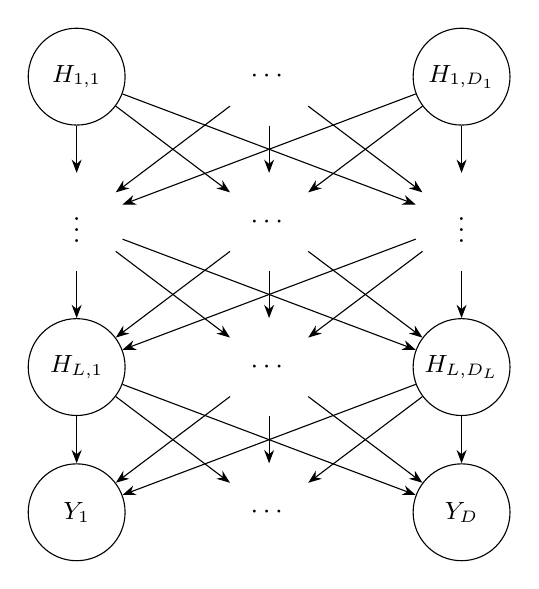
\begin{tikzpicture}[
      mycircle/.style={
         circle,
         draw=black,
         % fill=gray,
         fill opacity = 0.3,
         text opacity=1,
         inner sep=1pt,
         minimum size=35pt,
         font=\small},
      myarrow/.style={-Stealth},
      node distance=0.6cm and 1.2cm,
      node/.style={circle, draw, minimum size=35pt}
      ]
\node[mycircle            ] (y1) {$Y_1$};
\node[  circle,right=of y1,minimum size=35pt] (yd) {$\cdots$};
\node[mycircle,right=of yd] (yD) {$Y_D$};

\node[mycircle,above=of y1             ] (hL1) {$H_{L,1}$};
\node[  circle,above=of yd,right=of hL1,minimum size=35pt] (hLd) {$\cdots$};
\node[mycircle,above=of yD,right=of hLd] (hLD) {$H_{L,D_L}$};

\node[  circle,above=of hL1             ,minimum size=35pt] (hl1) {$\vdots$};
\node[  circle,above=of hLd,right=of hl1,minimum size=35pt] (hld) {$\cdots$};
\node[  circle,above=of hLD,right=of hld,minimum size=35pt] (hlD) {$\vdots$};

\node[mycircle,above=of hl1             ] (h11) {$H_{1,1}$};
\node[  circle,above=of hld,right=of h11,minimum size=35pt] (h1d) {$\cdots$};
\node[mycircle,above=of hld,right=of h1d] (h1D) {$H_{1,D_1}$};

\foreach \i/\j in {% start node/end node
      hL1/y1, hL1/yd, hL1/yD,
      hLd/y1, hLd/yd, hLd/yD,
      hLD/y1, hLD/yd, hLD/yD,
      hl1/hL1,hl1/hLd,hl1/hLD,
      hld/hL1,hld/hLd,hld/hLD,
      hlD/hL1,hlD/hLd,hlD/hLD,
      h11/hl1,h11/hld,h11/hlD,
      h1d/hl1,h1d/hld,h1d/hlD,
      h1D/hl1,h1D/hld,h1D/hlD}
       \draw[myarrow] (\i) -- node {} (\j);

\end{tikzpicture}
\begin{minipage}{0.85\textwidth}
\caption{A directed acyclic graph depicting a deep Gaussian process with 
$L$ hidden layers. Each arrow represents a Gaussian process with scalar 
output.}
\end{minipage}
\label{fig:deepgp}
\end{figure}






\subsection{Finite representation}

For $Y \in \mathbb{R}^{N \times D}$ and $X\in \mathbb{R}^{N\times Q}$,
then we have 
\[
Y_d \ind N(m_{1,d}(h_1), K_{1,d}(h_1,h_1))
\]
where 
$m_{1,d}(h_1)$ is the mean function evaluated at the output values for 
hidden layer 1, i.e. $h_{1,,1},\ldots,h_{1,,N}$ where $h_{1,,n}\in \mathcal{H}_1$
is the hidden layer 1 value associated with observation $n$, and 
$K_{1,d}(h_1,h_1)$ is the covariance matrix with $n,n'$-element
$k_{1,d}(h_{1,n},h_{1,n'})$.


\subsection{Mean and covariance functions}

Since each arrow in Figure \ref{fig:deepgp} represents a GP, 
we must select a mean and covariance function for each of these GPs. 
\cite{damianou2013deep} chose the *automatic relevance determination* (ARD) 
kernel
\[
k(h_{\ell,,n},h_{\ell,,n'}) = 
\sigma^2_{ard} \exp\left(-\frac{1}{2} \sum_{d=1}^{M_\ell} \omega_d \left[ h_{\ell,,n} - h_{\ell,,n'} \right]^2\right)
\]
with parameters $\sigma^2_{ard},\omega_1,\ldots,\omega_{M_\ell} > 0$.
This kernel is anisotropic because the dimensions are given different weights
as determined by $\omega_d$.
If $\omega_d \approx 0$ (or at least much smaller than the remaining $\omega$, 
then dimension $d$ provides almost no contribution to the correlation between
observations.

\cite{dunlop2018deep} use a covariance function constructed following 
\cite{paciorek2004nonstationary} who provide a general approach to constructing
nonstationary covariance kernels from stationary kernels.




\section{Inference}

\subsection{Model comparison}

Within the DGP framework,
we have the following model comparison issues:

\begin{itemize}
\item How many layers $L$ should there be?
\item What should the dimension be for layer $\ell$, $M_\ell$?
\end{itemize}
Ideally, we would use the marginal likelihood, 
i.e. $p(y|L,M_1,\ldots,M_L)$, to help us decide how many layers there should be
and how many dimensions per layer.
Methods that aim at estimating the marginal likelihood,
e.g. through a variational lower bound on the marginal likelihood \citep{damianou2013deep},
could be used for model comparison purposes.

\subsection{Parameter estimation}

Suppose we have selected a given DGP with $L$ layers and $M_1,\ldots,M_L$ 
dimensions for layers $1$ to $L$ respectively.
This DGP has $M=\sum_{\ell=1}^L M_\ell$ individual GPs, 
see Figure \ref{fig:deepgp}.

Each individual GP has a set of parameters defining its mean function $m$ and 
covariance function $k$. 


\bibliography{deepgp}

\end{document}